\documentclass[./project-report/src/latex/project-report.tex]{subfiles}

\begin{document}

\maketitle

\section{Testing TODO}

\subsection{Investigation}

\subsubsection{test\_model module}
\label{sec:test_model-module}

The test\_model module is contained within the frames package, and contains tkinter frames for testing the trained Artificial Neural Network models for each dataset. 
For each training dataset that an Artificial Neural Network is trained on, there is a corresponding test dataset with completely new images to be tested on to judge 
the performance of the trained model. As fewer images are needed for testing than for training, the Cat dataset only has 50 test images (compared to the 209 images 
for training) and the MNIST dataset only has 10,000 test images (compared to the 60,000 images for training).
Each frame displays the results of the testing along with a random selection of incorrect and correct predictions.

\inputminted{python}{./school_project/frames/test_model.py}

Which outputs the following for the MNIST dataset:

\pagebreak

\begin{figure}[h!]
\centering
\frame{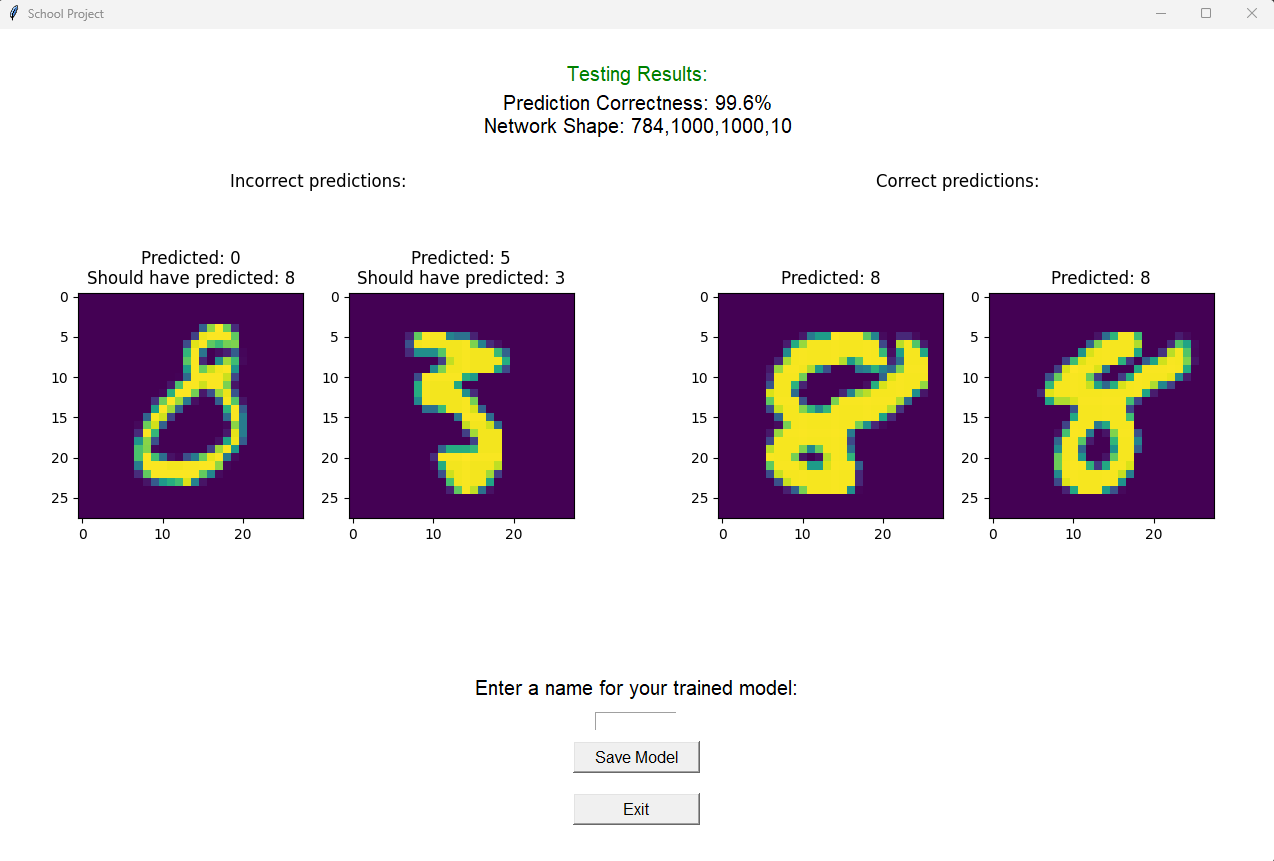
\includegraphics[width=1\textwidth]{./project-report/src/images/test-mnist-frame.png}}
\end{figure}

And outputs the following for the Cat Recognition dataset:

\pagebreak

\begin{figure}[h!]
\centering
\frame{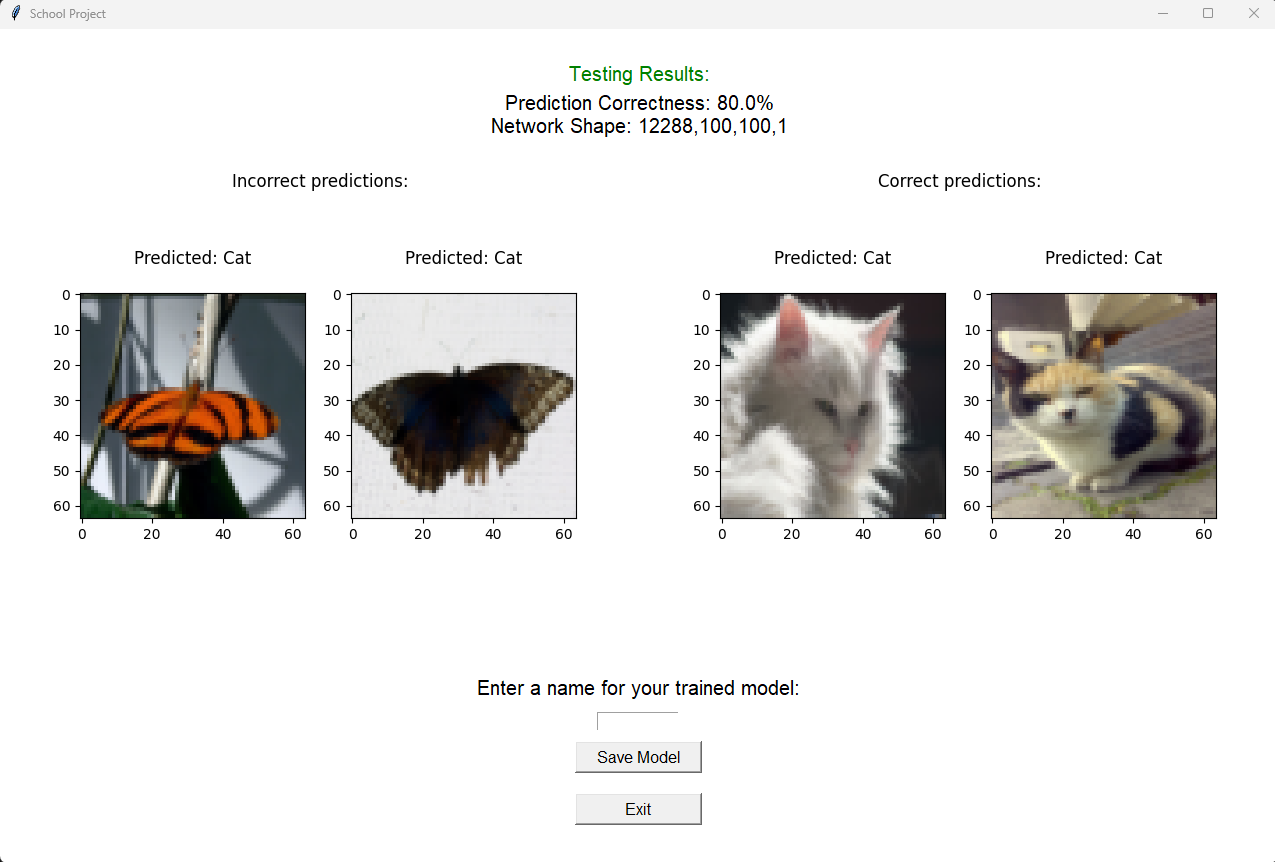
\includegraphics[width=1\textwidth]{./project-report/src/images/test-cat-recognition-frame.png}}
\end{figure}

And outputs the following for the XOR dataset:

\pagebreak

\begin{figure}[h!]
\centering
\frame{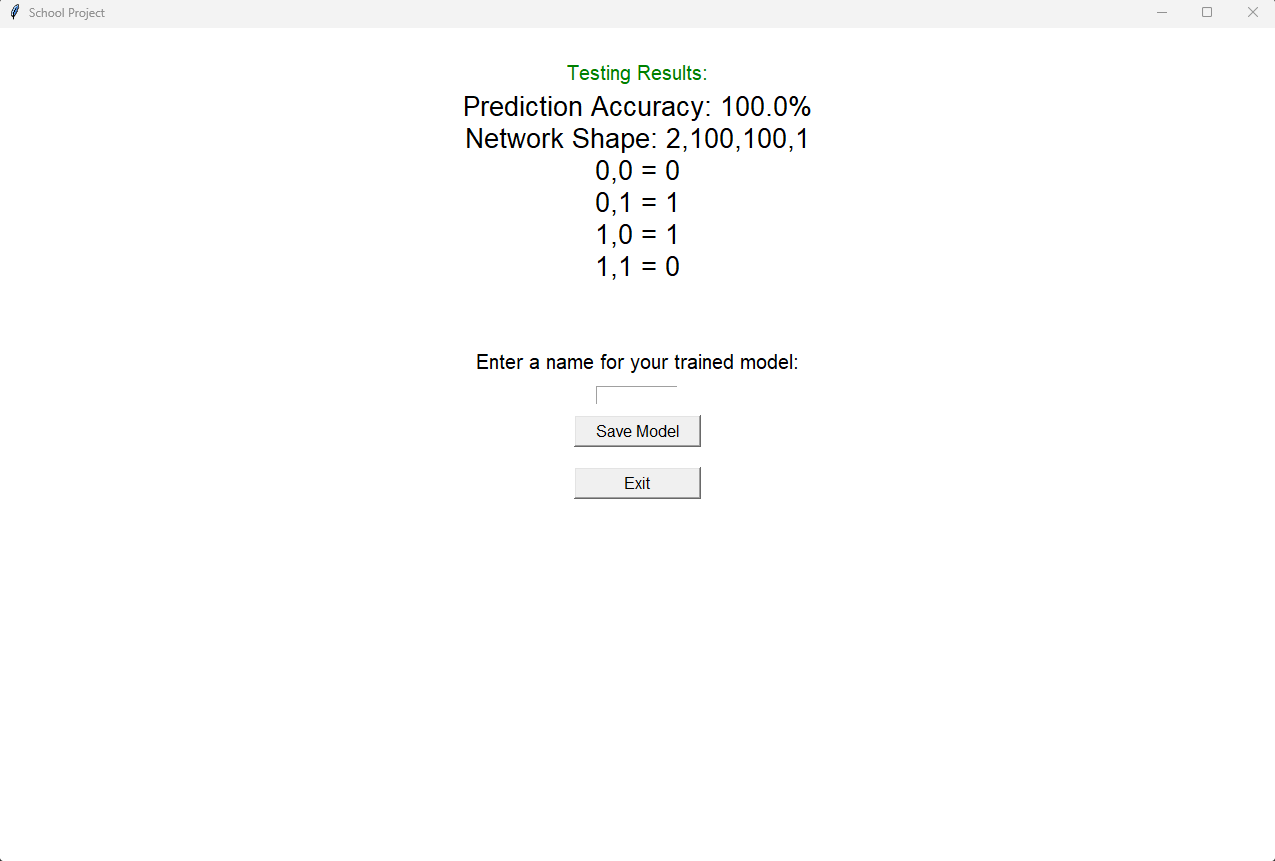
\includegraphics[width=1\textwidth]{./project-report/src/images/test-xor-frame.png}}
\end{figure}

\subsubsection{Effects of Hyper-Parameters}
\label{sec:effects-of-hyper-parameters}

For the following investigations, I utilised Jupyter Notebook and have displayed the results below:

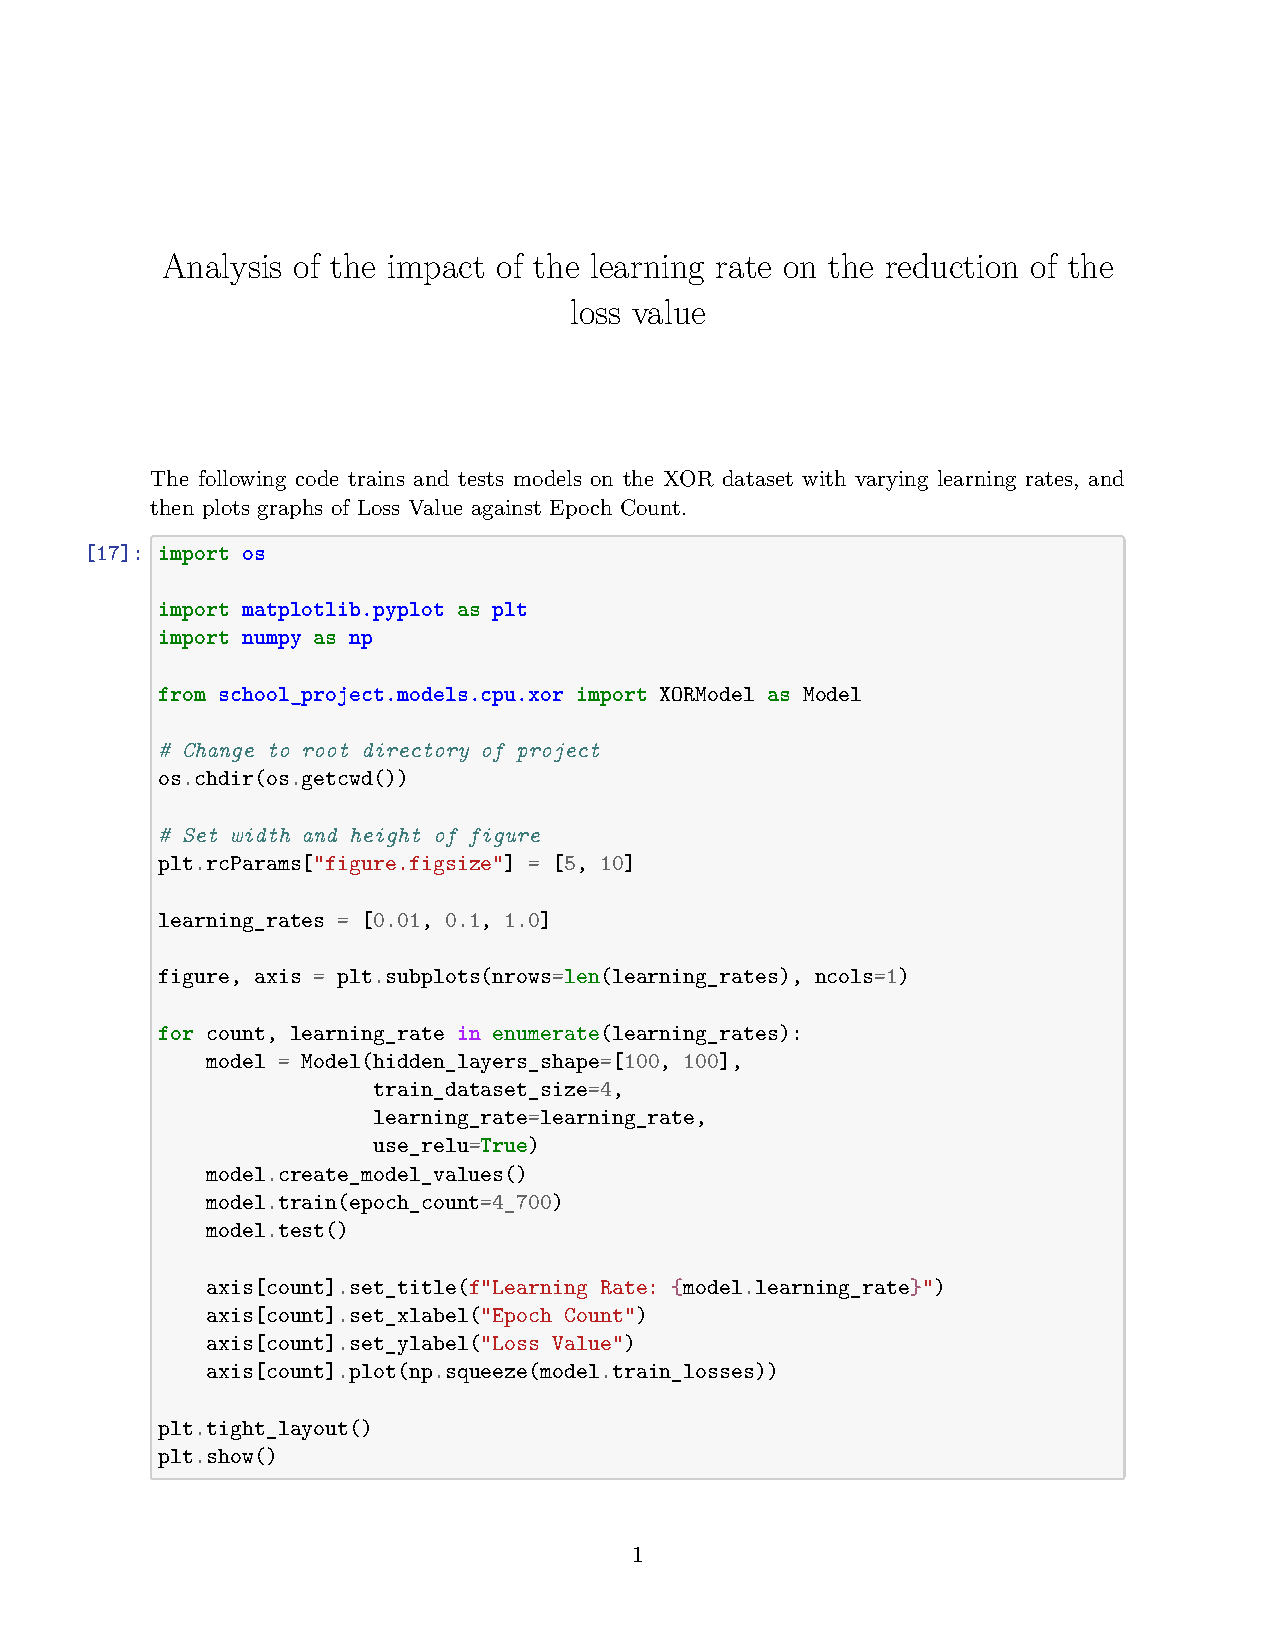
\includepdf[pages=-, pagecommand={\thispagestyle{plain}}, scale=0.9]{./project-report/src/pdfs/learning-rate-analysis.pdf}
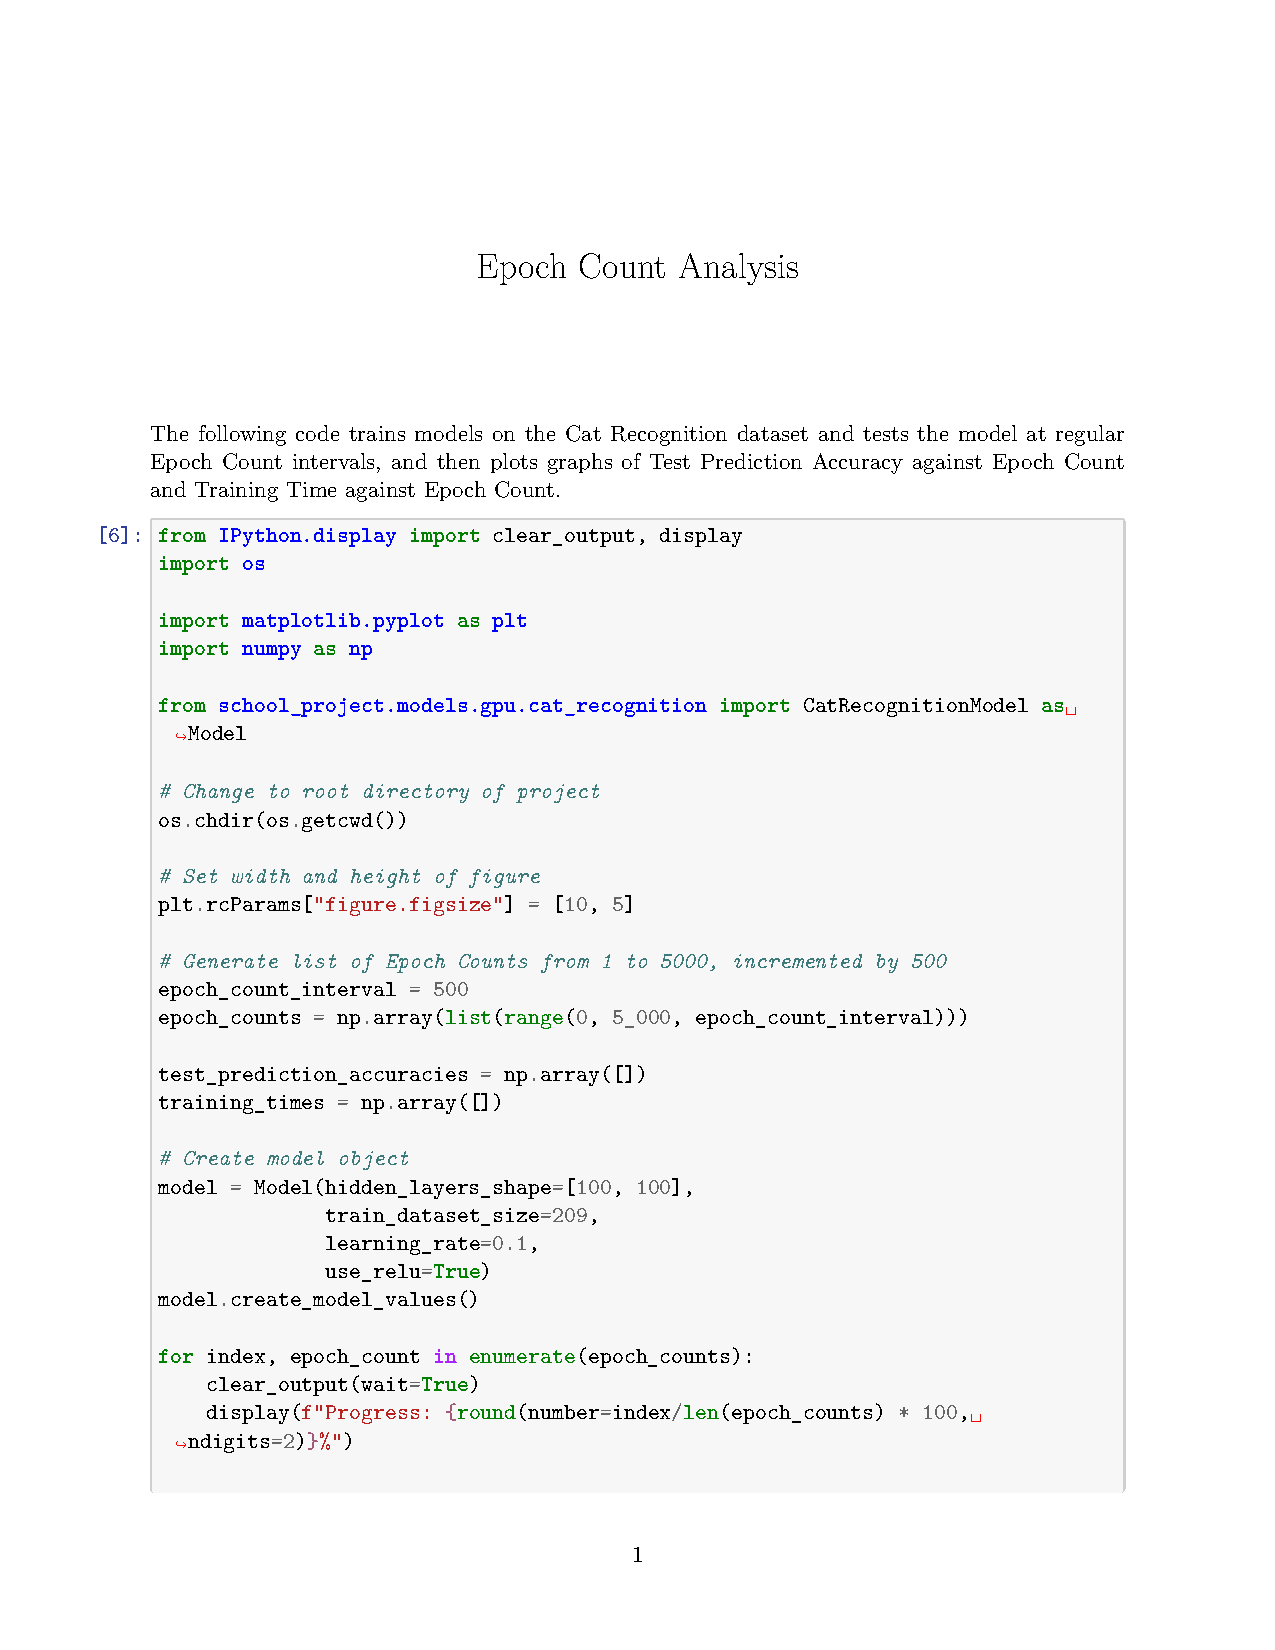
\includepdf[pages=-, pagecommand={\thispagestyle{plain}}, scale=0.9]{./project-report/src/pdfs/epoch-count-analysis.pdf}
\label{sec:train-dataset-size-analysis}
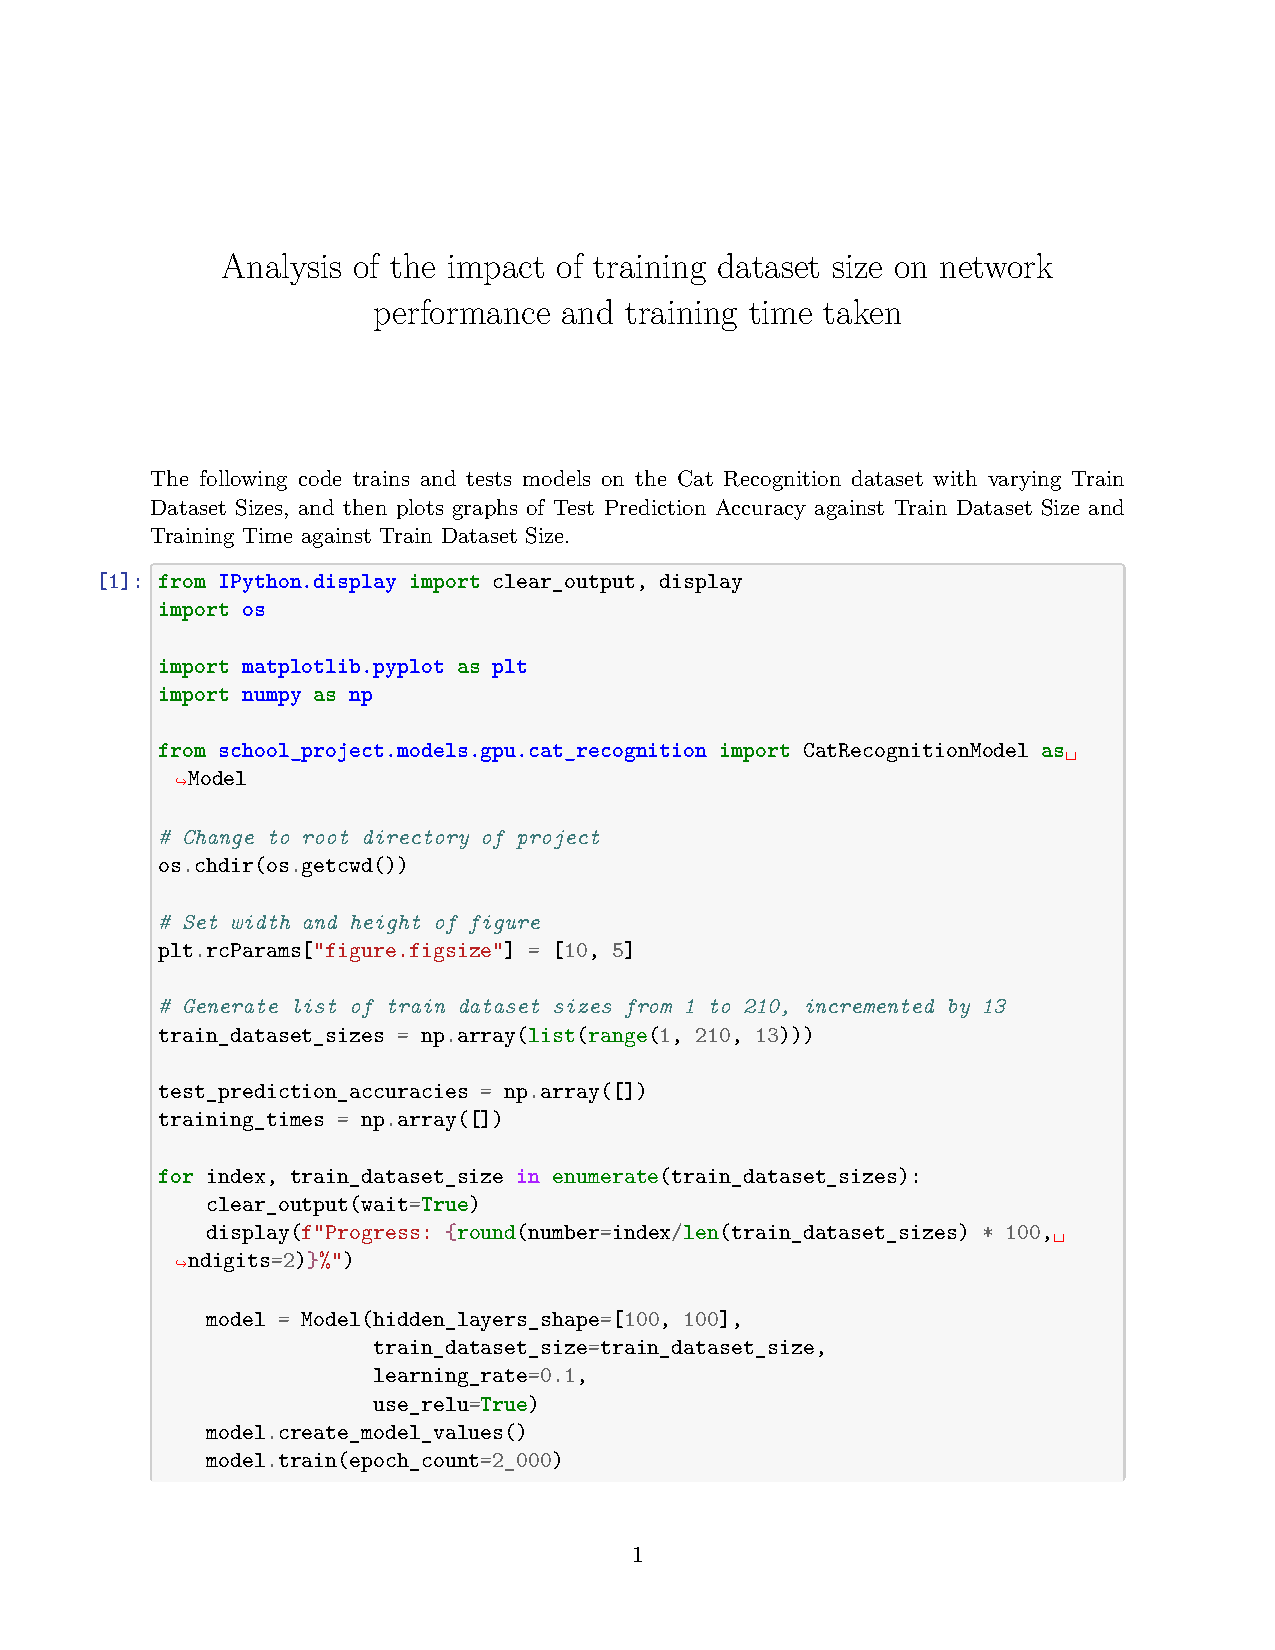
\includepdf[pages=-, pagecommand={\thispagestyle{plain}}, scale=0.9]{./project-report/src/pdfs/train-dataset-size-analysis.pdf}
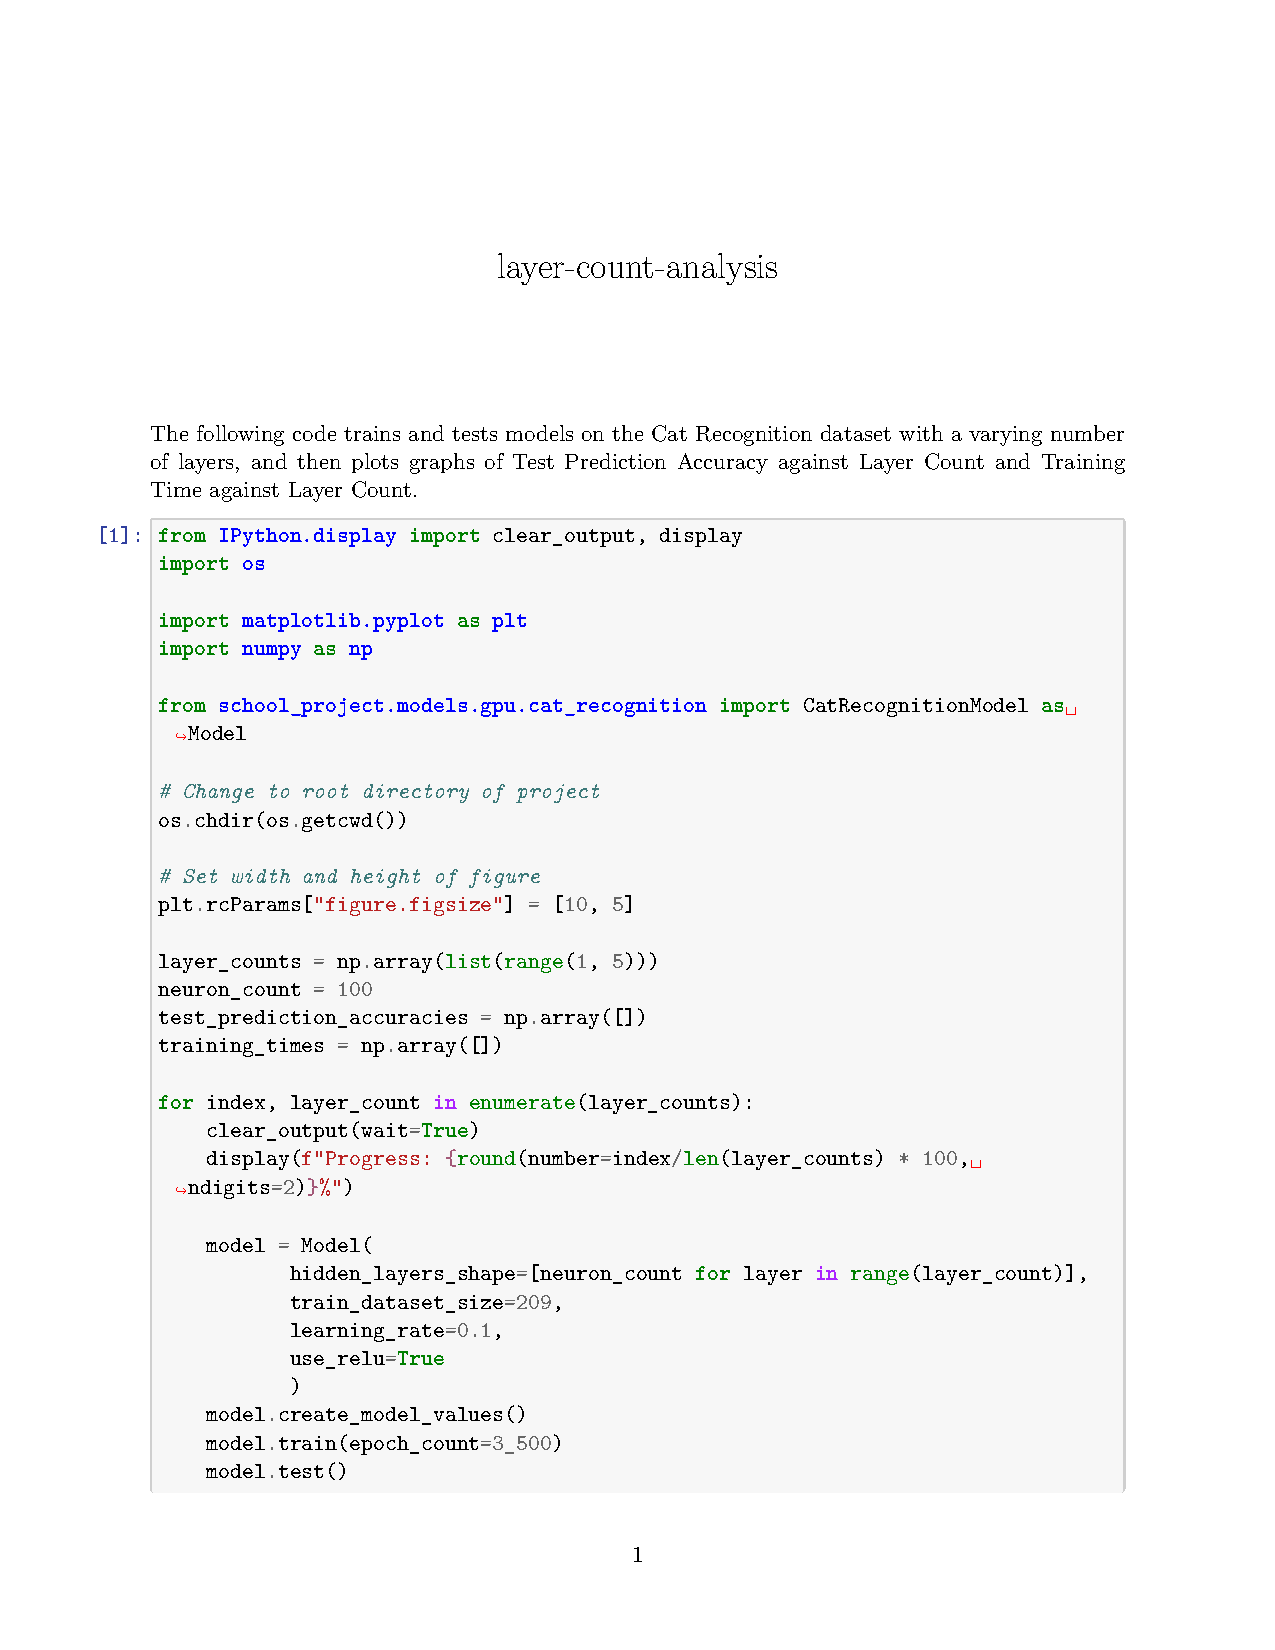
\includepdf[pages=-, pagecommand={\thispagestyle{plain}}, scale=0.9]{./project-report/src/pdfs/layer-count-analysis.pdf}
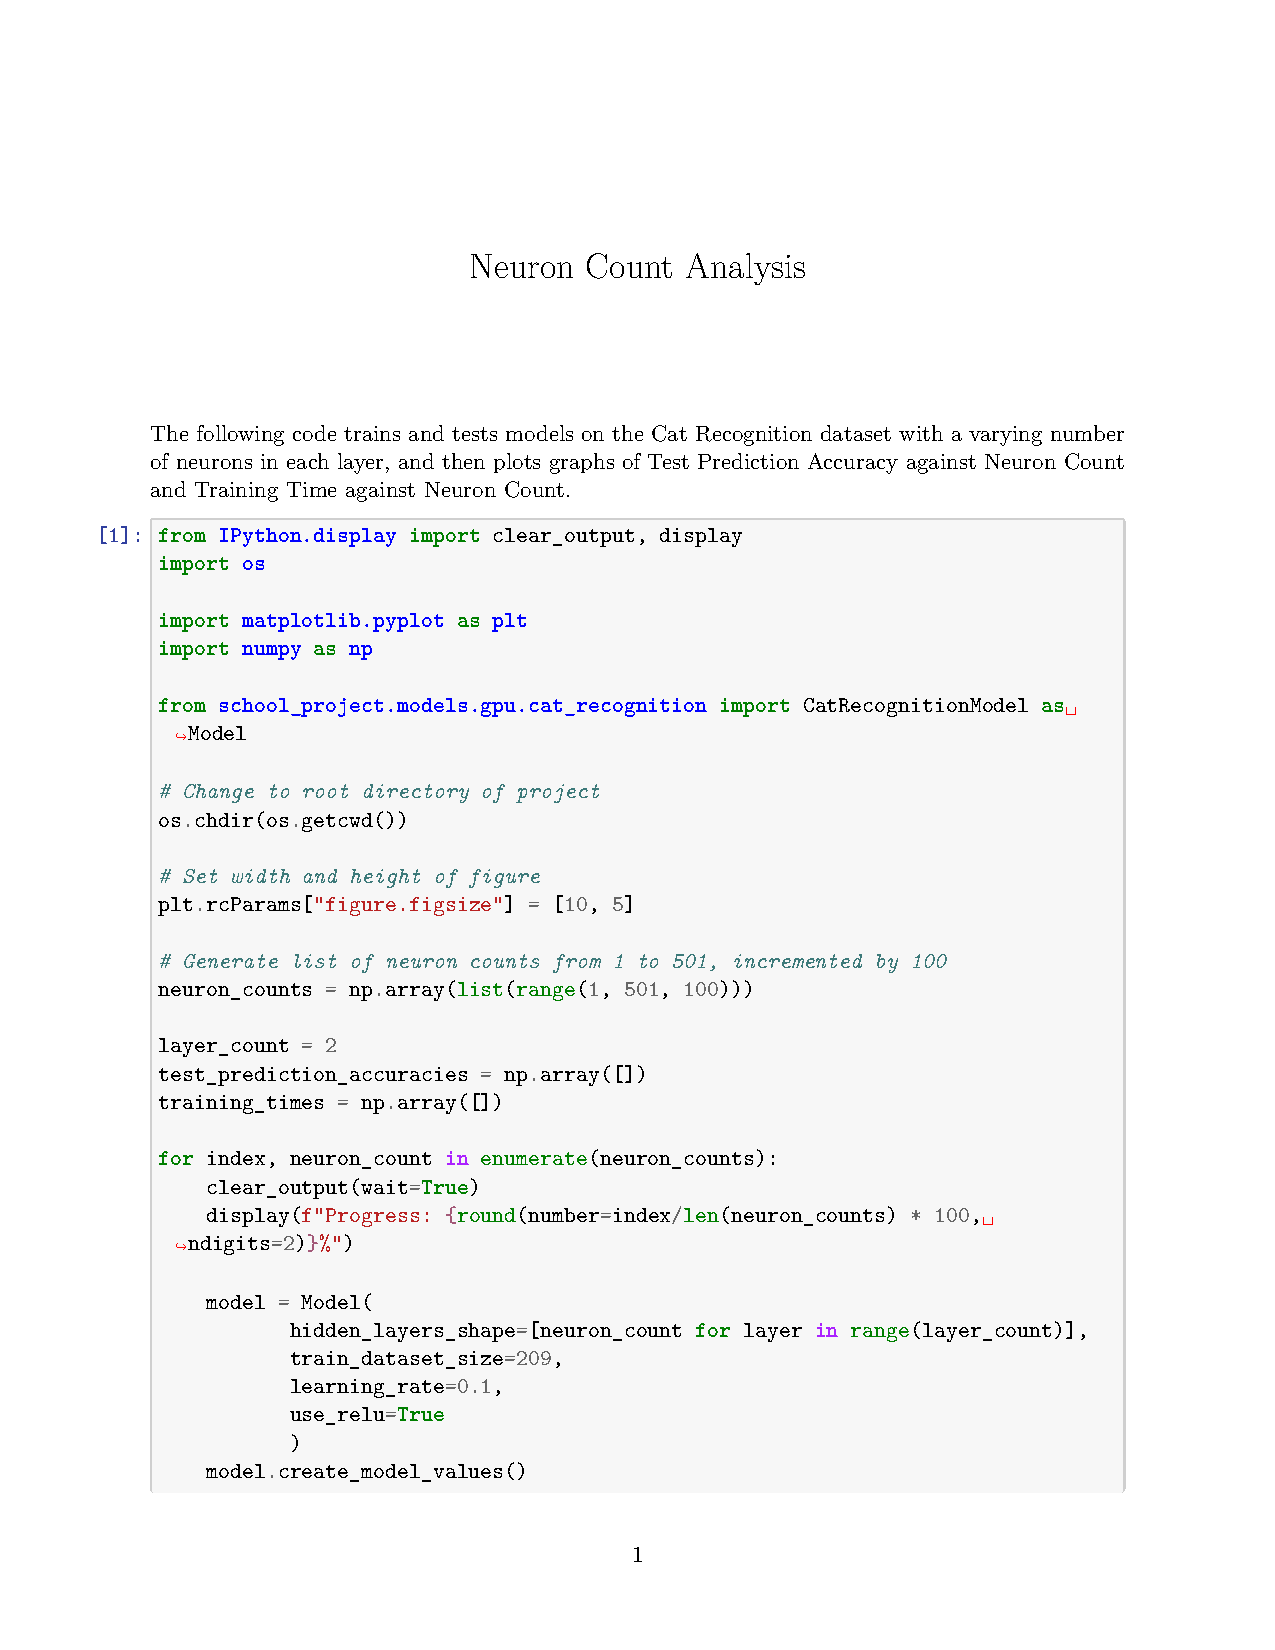
\includepdf[pages=-, pagecommand={\thispagestyle{plain}}, scale=0.9]{./project-report/src/pdfs/neuron-count-analysis.pdf}
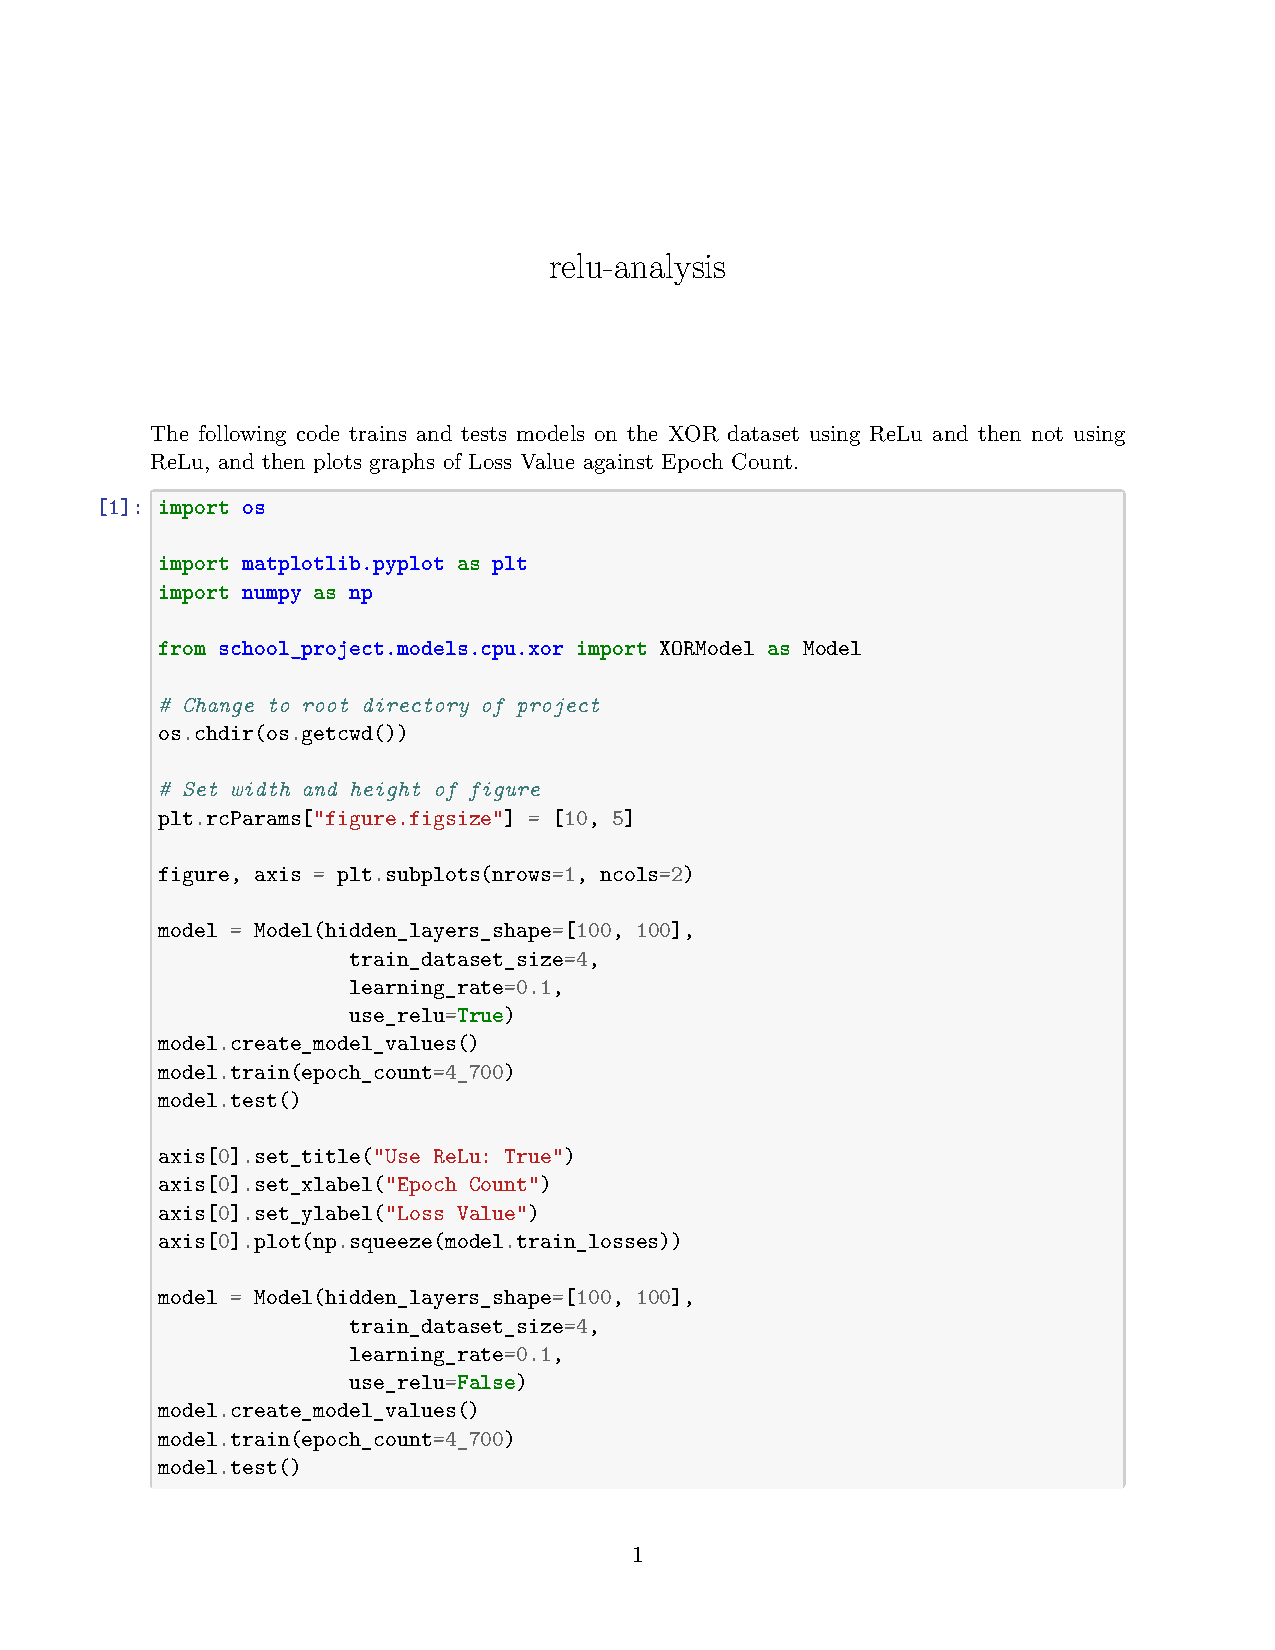
\includepdf[pages=-, pagecommand={\thispagestyle{plain}}, scale=0.9]{./project-report/src/pdfs/relu-analysis.pdf}
\label{sec:cpu-vs-gpu-analysis}
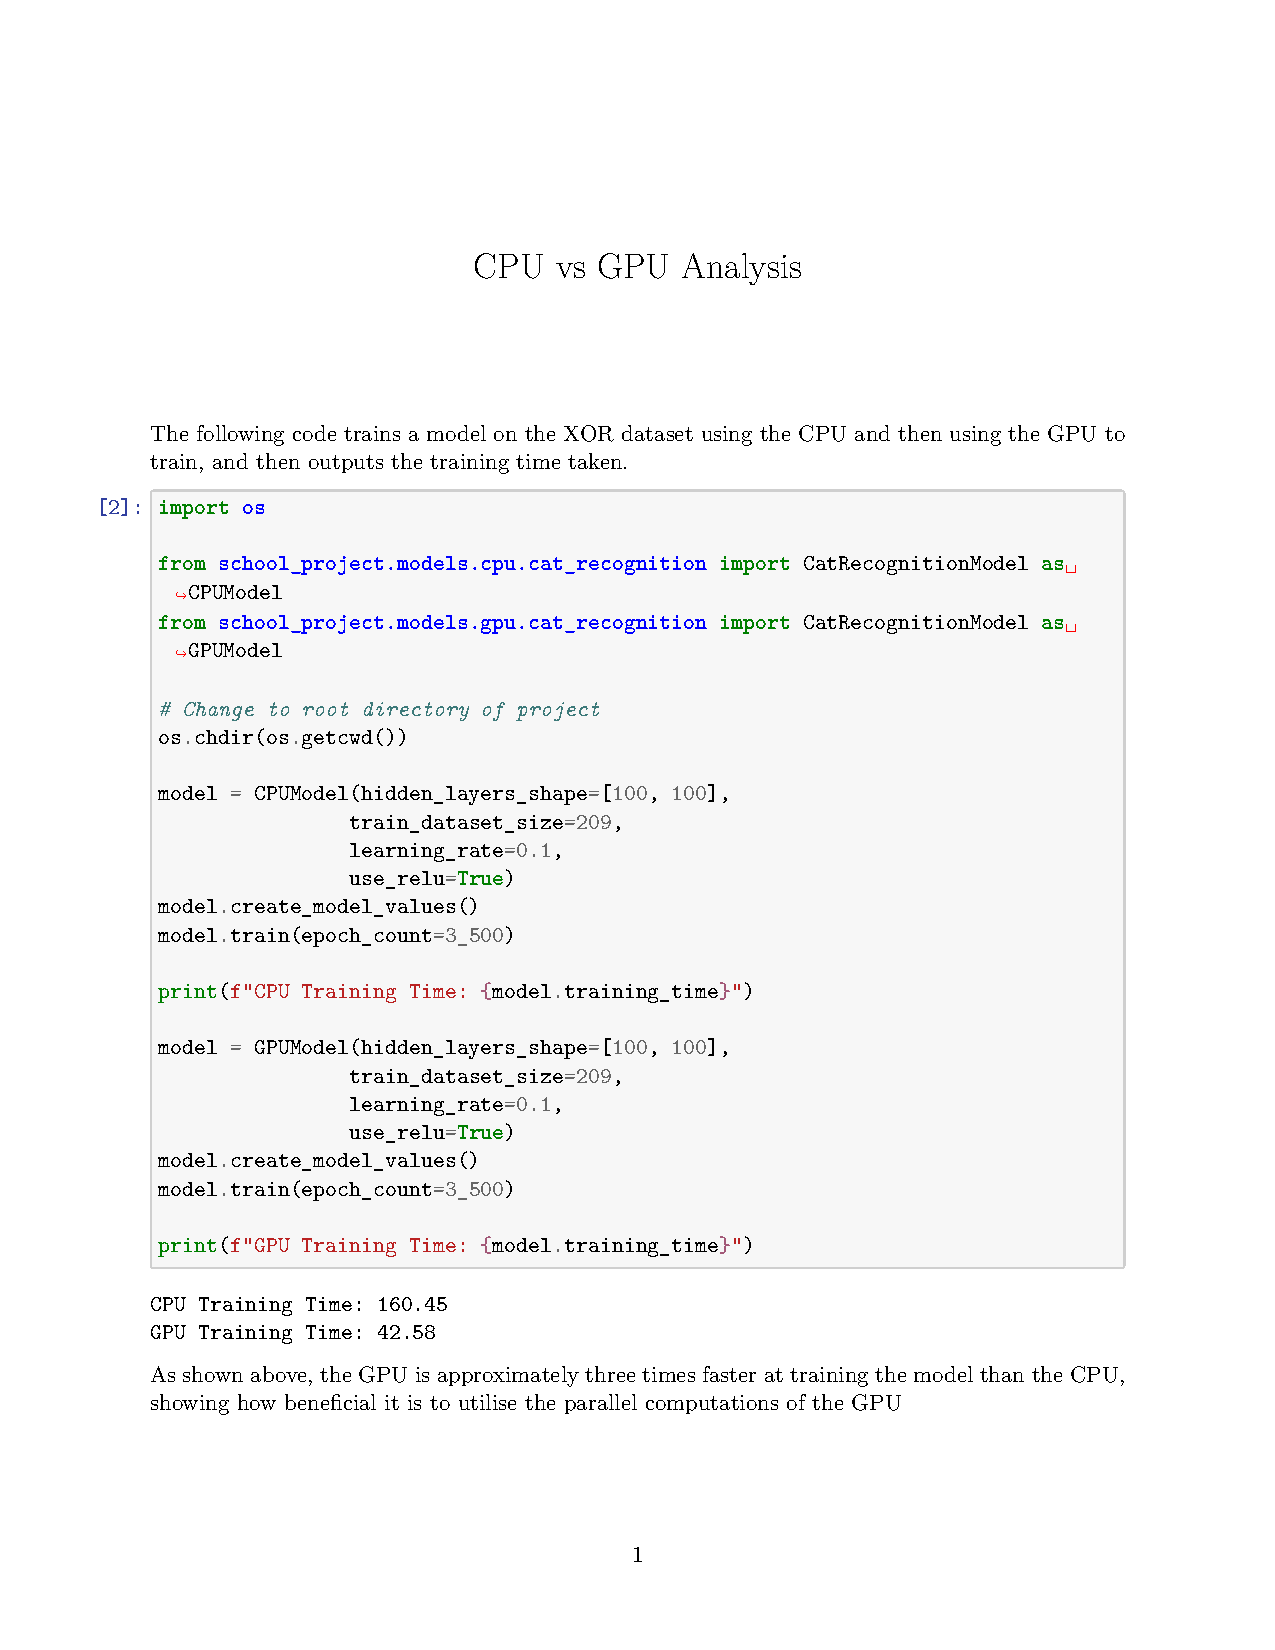
\includepdf[pages=-, pagecommand={\thispagestyle{plain}}, scale=0.9]{./project-report/src/pdfs/cpu-vs-gpu-analysis.pdf}

\subsection{Manual Testing}

\subsubsection{Input Validation Testing} % See table on teams

The following tests check the input validation of each frames' inputs.

\begin{itemize}
    \item Hyper Parameter Frame:
    \label{sec:hyper-parameter-frame-input-validation}
    \begin{itemize}
        \item Use GPU Validation:
            \begin{itemize}
                \item Description: Select Use GPU checkbox without a GPU present.
                \item Expected Result: The exception should be handled and a useful error message should be displayed.
                \item Actual Result: Expected Result
                \item Test Status: Pass
                \item Evidence:
                    \begin{figure}[h!]
                    \centering
                    \frame{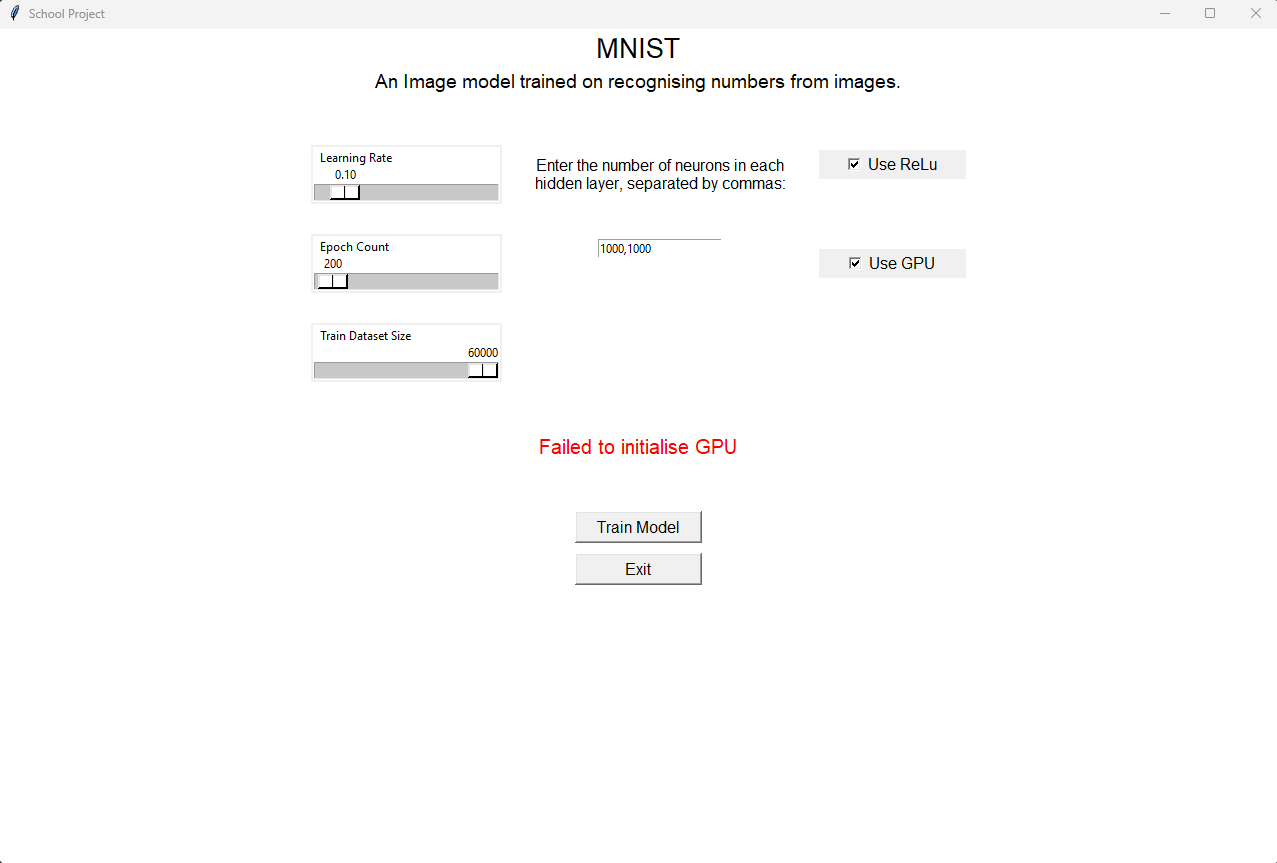
\includegraphics[width=1\textwidth]{./project-report/src/images/create-model-use-gpu-validation.png}}
                    \end{figure}

                    Link to video evidence: \url{https://github.com/mcttn22/school-project/blob/main/project-report/input-validation-testing-videos.md/#use-gpu-validation}
            \end{itemize}

        \pagebreak

        \item Hidden Layers Shape Validation:
            \begin{itemize}
                \item Description: Enter an invalid hidden layers shape.
                \item Data Value: "test"
                \item Data Type: Erroneous
                \item Expected Result: The exception should be handled and a useful error message should be displayed.
                \item Actual Result: Expected Result
                \item Test Status: Pass
                \item Evidence:
                    \begin{figure}[h!]
                    \centering
                    \frame{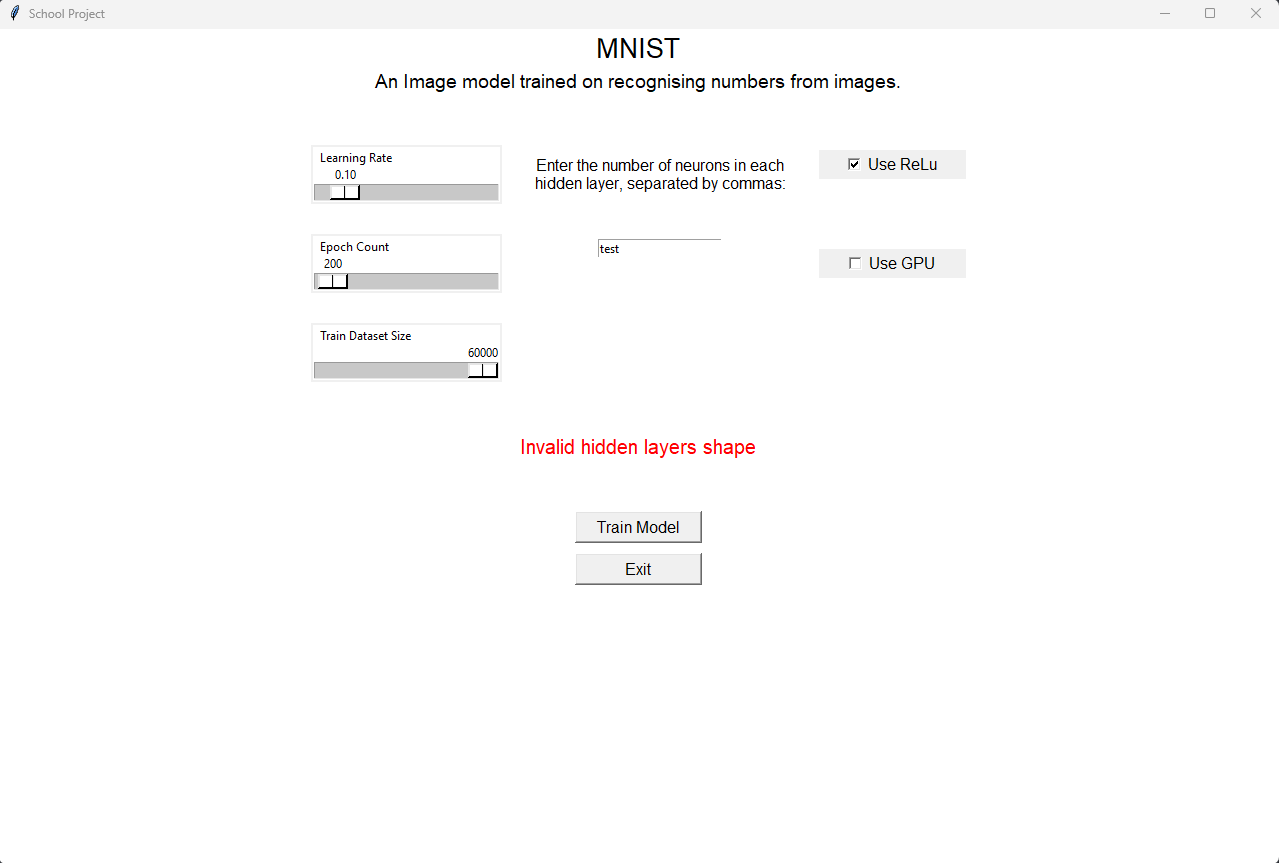
\includegraphics[width=1\textwidth]{./project-report/src/images/hidden-layers-shape-input-validation.png}}
                    \end{figure}

                    Link to video evidence: \url{https://github.com/mcttn22/school-project/blob/main/project-report/input-validation-testing-videos.md/#hidden-layers-shape-validation}
            \end{itemize}
    \end{itemize}

    \pagebreak

    \item Load Model Frame:
    \label{sec:load-model-frame-input-validation}
    \begin{itemize}
        \item Use GPU Validation:
            \begin{itemize}
            \item Description: Select Use GPU checkbox without a GPU present.
            \item Expected Result: The exception should be handled and a useful error message should be displayed.
            \item Actual Result: Expected Result
            \item Test Status: Pass
            \item Evidence:
                \begin{figure}[h!]
                \centering
                \frame{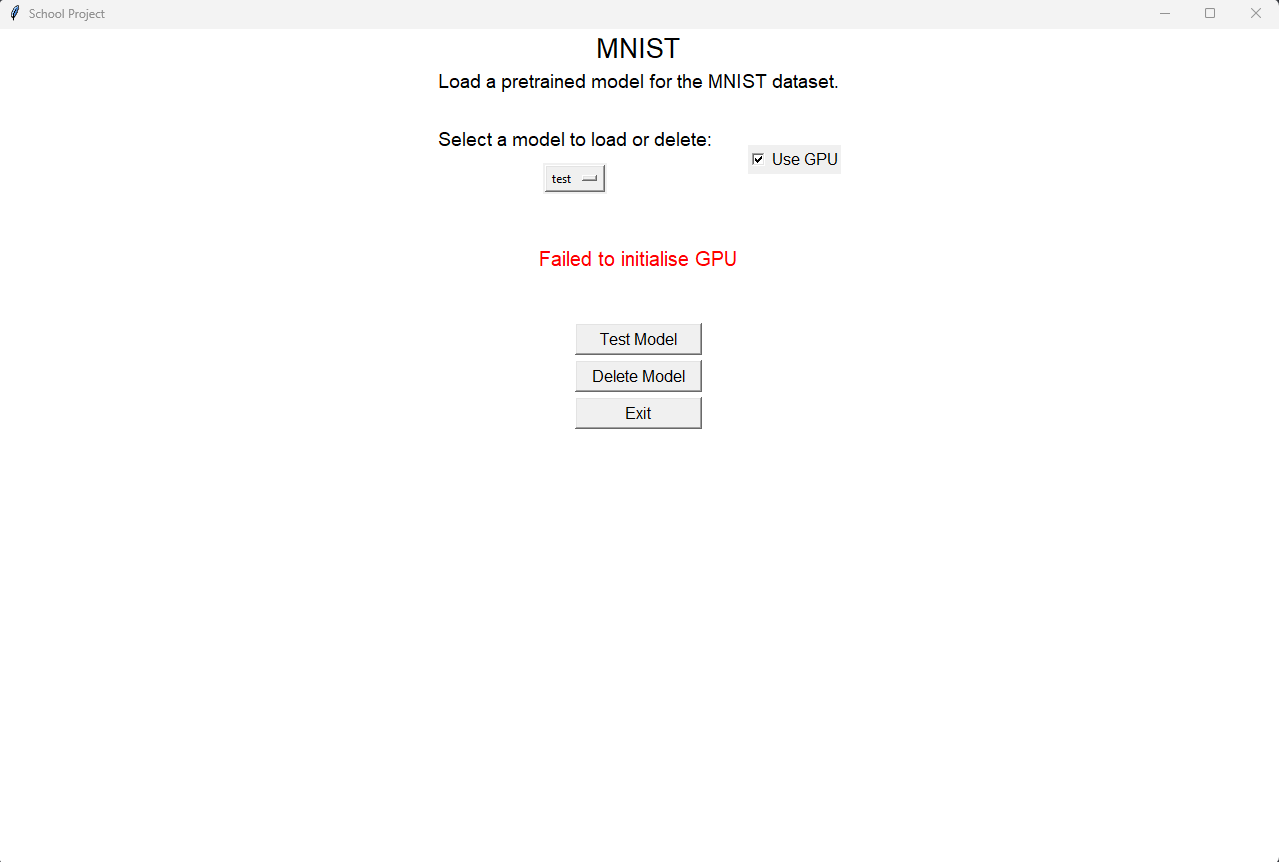
\includegraphics[width=1\textwidth]{./project-report/src/images/load-model-use-gpu-validation.png}}
                \end{figure}

                Link to video evidence: \url{https://github.com/mcttn22/school-project/blob/main/project-report/input-validation-testing-videos.md/#hidden-layers-shape-validation}
            \end{itemize}
    \end{itemize}

    \pagebreak

    \item Test Frames:
    \label{sec:test-frames-input-validation}
    \begin{itemize}
        \item Taken Trained Model Name Validation:
            \begin{itemize}
                \item Description: Try to save a trained model with an already taken name.
                \item Data Value: "test"
                \item Data Type: Erroneous
                \item Expected Result: The exception should be handled and a useful error message should be displayed.
                \item Actual Result: Expected Result
                \item Test Status: Pass
                \item Evidence:
                    \begin{figure}[h!]
                    \centering
                    \frame{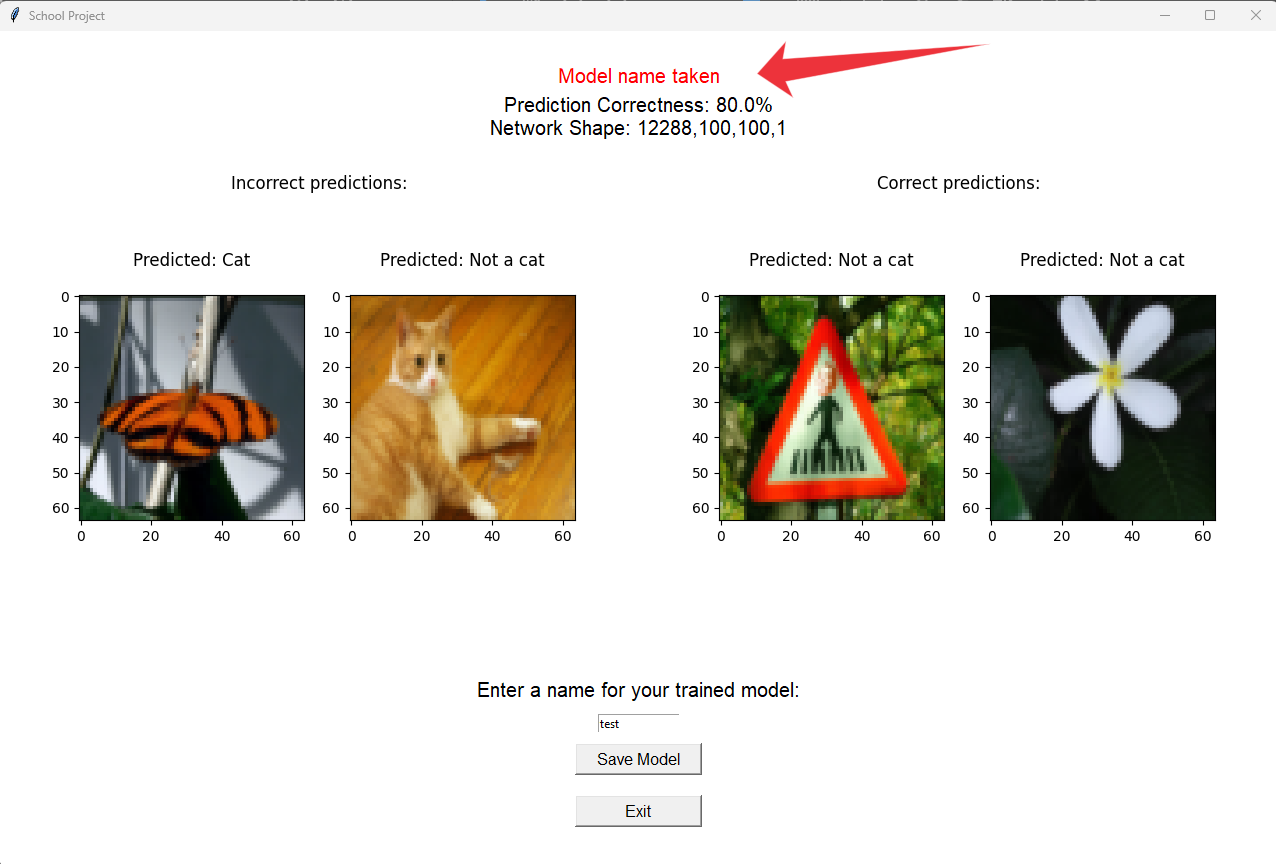
\includegraphics[width=1\textwidth]{./project-report/src/images/taken-trained-model-name-input-validation.png}}
                    \end{figure}

                    Link to video evidence: \url{https://github.com/mcttn22/school-project/blob/main/project-report/input-validation-testing-videos.md/#hidden-layers-shape-validation}
            \end{itemize}

        \pagebreak
        
        \item Empty Trained Model Name Validation:
            \begin{itemize}
                \item Description: Try to save a trained model with blank name.
                \item Data Value: ""
                \item Data Type: Erroneous
                \item Expected Result: The exception should be handled and a useful error message should be displayed.
                \item Actual Result: Expected Result
                \item Test Status: Pass
                \item Evidence:
                    \begin{figure}[h!]
                    \centering
                    \frame{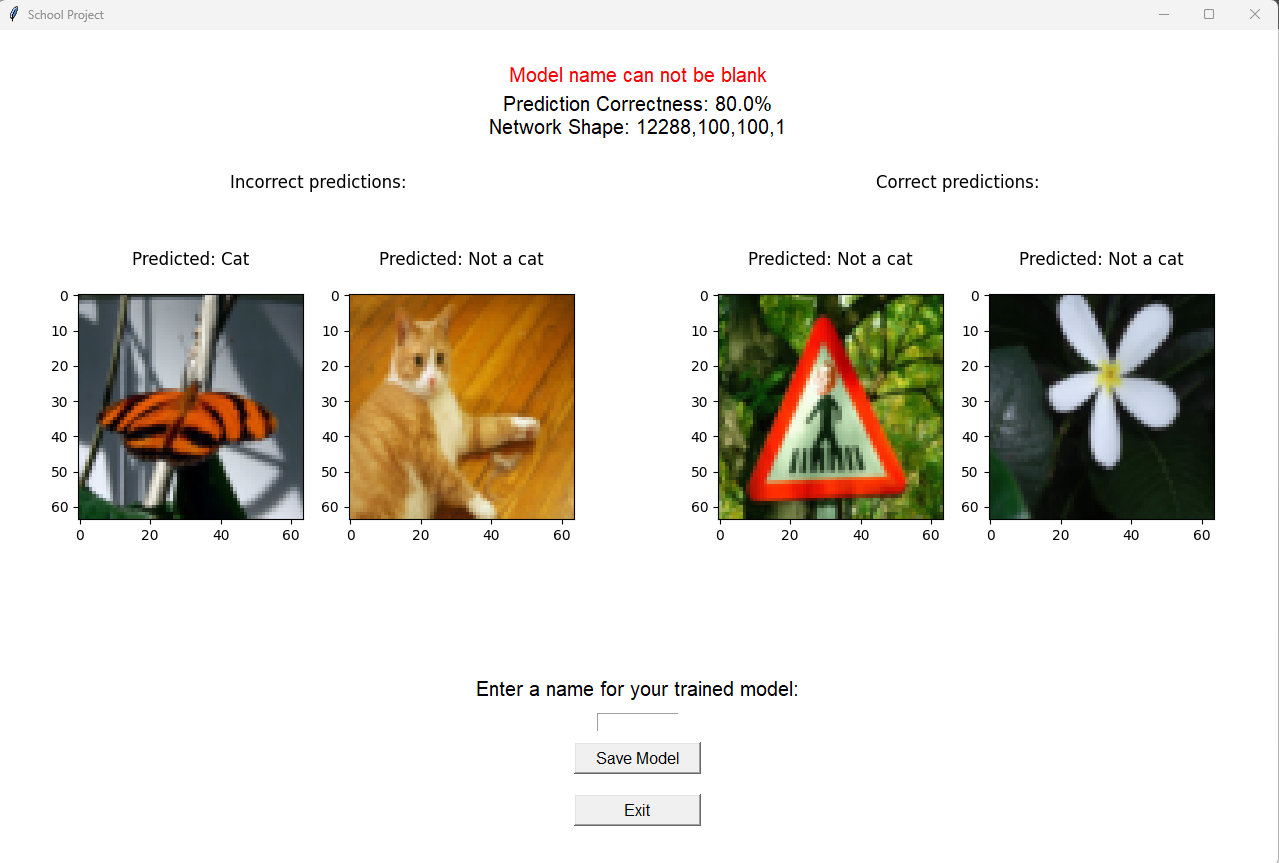
\includegraphics[width=1\textwidth]{./project-report/src/images/empty-trained-model-name-input-validation.png}}
                    \end{figure}

                    Link to video evidence: \url{https://github.com/mcttn22/school-project/blob/main/project-report/input-validation-testing-videos.md/#hidden-layers-shape-validation}
            \end{itemize}
    \end{itemize}
\end{itemize}

\subsection{Automated Testing}

\subsubsection{Unit Tests}
\label{sec:unit-tests}

Within the test package, I have written the following unit tests for the utils subpackage of both the cpu and gpu subpackage of the models package. Similarly to the code for the cpu 
and gpu subpackage, it is only worth showing the code for the cpu version as both are very similar in functionality.

\begin{itemize}
    \item test\_model.py module:
        \inputminted{python}{./school_project/test/models/cpu/utils/test_model.py}

        \pagebreak

    \item test\_tools.py module:
        \inputminted{python}{./school_project/test/models/cpu/utils/test_tools.py}
\end{itemize}

\subsubsection{GitHub Automated Testing}

With the following configuration programmed in the .github/workflows/tests.yml file, the unit tests are run automatically on GitHub servers after each commit that is pushed to GitHub, 
and the status of the tests (either passing or failing) can be viewed on the repository's page. This automatic testing allows for a faster workflow and allows me to identify which changes 
(commits) cause issues within the code, allowing for easier maintenance of the project.

\inputminted{yaml}{./.github/workflows/tests.yml}

\subsubsection{Docker}

I also provide a basic Dockerfile and instructions for its use in the README.md file, so that the project can be quickly run and tested in Docker containers. Below 
shows the contents of the basic Dockerfile:

\inputminted{docker}{./Dockerfile}

\end{document}